\documentclass{vgtc}     

\ifpdf%                                % if we use pdflatex
  \pdfoutput=1\relax                   % create PDFs from pdfLaTeX
  \pdfcompresslevel=9                  % PDF Compression
  \pdfoptionpdfminorversion=7          % create PDF 1.7
  \ExecuteOptions{pdftex}
  \usepackage{graphicx}                % allow us to embed graphics files
  \DeclareGraphicsExtensions{.pdf,.png,.jpg,.jpeg} % for pdflatex we expect .pdf, .png, or .jpg files
\else%                                 % else we use pure latex
  \ExecuteOptions{dvips}
  \usepackage{graphicx}                % allow us to embed graphics files
  \DeclareGraphicsExtensions{.eps}     % for pure latex we expect eps files
\fi%

%% it is recomended to use ``\autoref{sec:bla}'' instead of ``Fig.~\ref{sec:bla}''
\graphicspath{{figures/}{pictures/}{images/}{./}} % where to search for the images

\usepackage{microtype}                 % use micro-typography (slightly more compact, better to read)
\PassOptionsToPackage{warn}{textcomp}  % to address font issues with \textrightarrow
\usepackage{textcomp}                  % use better special symbols
\usepackage{mathptmx}                  % use matching math font
\usepackage{times}                     % we use Times as the main font
\renewcommand*\ttdefault{txtt}         % a nicer typewriter font
\usepackage{cite}                      % needed to automatically sort the references
\usepackage{tabu}                      % only used for the table example
\usepackage{booktabs}                  % only used for the table example
%% We encourage the use of mathptmx for consistent usage of times font
%% throughout the proceedings. However, if you encounter conflicts
%% with other math-related packages, you may want to disable it.


%% If you are submitting a paper to a conference for review with a double
%% blind reviewing process, please replace the value ``0'' below with your
%% OnlineID. Otherwise, you may safely leave it at ``0''.
\onlineid{0}

%% declare the category of your paper, only shown in review mode
\vgtccategory{Research}

%% allow for this line if you want the electronic option to work properly
\vgtcinsertpkg

%% In preprint mode you may define your own headline.
%\preprinttext{To appear in an IEEE VGTC sponsored conference.}

%% Paper title.

\usepackage{amsmath}
\usepackage{graphicx}
\usepackage{balance}  % for  \balance command ON LAST PAGE  (only there!)
\usepackage{adjustbox}
\usepackage{footmisc}
\usepackage{soul}
\usepackage{hyperref}
\usepackage{enumitem}
\usepackage{multirow}
\usepackage{listings}
\usepackage{cleveref}
\usepackage{array}
\usepackage{tabularx}
\usepackage{booktabs} % For formal tables
\usepackage{xspace}
\usepackage{xcolor}
\usepackage{microtype}
\usepackage{subcaption}
\usepackage{balance}
\usepackage{mathtools}
\usepackage{scalerel}
%\usepackage{amssymb}
%\usepackage{tcolorbox}% http://ctan.org/pkg/tcolorbox
\usepackage{adjustbox}
%\usepackage{nopageno}
\usepackage{float}

\usepackage[noend]{algpseudocode}
\usepackage{algorithmicx,algorithm}


\pagenumbering{arabic}


\definecolor{darkgreen}{rgb}{0.15,0.55,0.15}
\definecolor{darkblue}{rgb}{0.1,0.1,0.5}
\definecolor{orange}{rgb}{1, 0.64, 0}
%\definecolor{blue}{rgb}{0.19,0.58,1}
\definecolor{blue}{rgb}{0.01,0.40,.8}
\definecolor{darkgreen}{rgb}{0.15,0.55,0.15}
\definecolor{mred}{rgb}{.80,.12,.30}
\definecolor{grey}{rgb}{0.5,0.5,0.5}
\definecolor{Purple}{rgb}{.75,0,.85}
\definecolor{light-gray}{gray}{0.95}
\definecolor{mid-gray}{gray}{0.85}
\definecolor{darkred}{rgb}{0.7,0.25,0.25}
\definecolor{rose}{rgb}{1.0, 0.01, 0.24}
\definecolor{lightyellow}{HTML}{FFD700}
\definecolor{lgreen}{HTML}{C2E9D7}
%\definecolor{rose}{rgb}{0.9, 0.13, 0.13}
\newcommand{\red}[1]{\textcolor{red}{#1}}
\newcommand{\darkgreen}[1]{\textcolor{darkgreen}{#1}}
\newcommand{\lightyellow}[1]{\textcolor{lightyellow}{#1}}
\newcommand{\grey}[1]{\textcolor{grey}{#1}}
\newcommand{\gray}[1]{\textcolor{grey}{#1}}
\newcommand{\rose}[1]{\textcolor{americanrose}{#1}}
\newcommand{\redtt}[1]{\textcolor{red}{\texttt{#1}}}
\newcommand{\green}[1]{\textcolor{green}{#1}}
\newcommand{\lgreen}[1]{\textcolor{lgreen}{#1}}
\newcommand{\blue}[1]{\textcolor{blue}{#1}}
\newcommand{\orange}[1]{\textcolor{orange}{#1}}
\newcommand{\highlight}[1]{{\setlength{\fboxsep}{1pt}\colorbox{yellow}{\textbf{\texttt{#1}}}}}
\newcommand{\ghighlight}[1]{{\setlength{\fboxsep}{1pt}\colorbox{lgreen}{\textbf{\texttt{#1}}}}}


%\newtcbox{\redbox}{on line,
%  colframe=white,colback=red!10!white,
%  height=1em,valign=bottom,
%  boxrule=0.5pt,arc=2pt,boxsep=0pt,left=2pt,right=2pt,top=1pt,bottom=1pt}
%\newtcbox{\bluebox}{on line,
%  colframe=white,colback=blue!10!white,
%  height=1em,valign=bottom,
%  boxrule=0.5pt,arc=2pt,boxsep=0pt,left=2pt,right=2pt,top=1pt,bottom=1pt}



\newcommand{\eat}[1]{}

\newcommand{\ititle}[1]{\vspace{2pt}\noindent\emph{#1}}
\newcommand{\stitle}[1]{\smallskip\noindent\textbf{#1}}
\newcommand{\sstitle}[1]{\noindent\textbf{#1}}
\newtheorem{theorem}{Theorem}

%% listing settings
\newlength{\listingindent}                %declare a new length
\setlength{\listingindent}{\parindent}    %make it a fixed version of \parindent
\lstset{escapeinside={<@}{@>}, language=SQL}
\lstset{xleftmargin=2em}

\lstset{
	language = SQL,
	showspaces=false,
	basicstyle=\ttfamily\scriptsize,
	commentstyle=\color{gray},
	mathescape=true,
	numbers=none,
    escapeinside={^}{^},
	captionpos=b,	
	float=tp,
	floatplacement=tbp,
	belowskip=-0.05em,
    breaklines=true,
    frame=tlrb,
    xleftmargin=0pt,xrightmargin=0pt
} 

\usepackage{tablefootnote}

\usepackage[LGRgreek]{mathastext}
\widowpenalty=10000
\clubpenalty=10000


\DeclarePairedDelimiter\ceil{\lceil}{\rceil}
\DeclarePairedDelimiter\floor{\lfloor}{\rfloor}


\newcommand{\papertext}[1]{#1}
\newcommand{\techreport}[1]{#1}


\newenvironment{myitemize}{\vspace{-0.1in}\begin{list}{\gray{$\bullet$}}{\renewcommand{\itemsep}{-0.0in}\renewcommand{\leftmargin}{0.15in}}}{\end{list}\vspace{-.1in}}

\newcommand{\spacing}[1]{\renewcommand{\baselinestretch}{#1}}


\renewcommand{\arraystretch}{1}

                    
\newtheorem{thm}{Theorem}
\newtheorem{example}{Example}
\newtheorem{definition}{Definition}
\newtheorem{problem}{Problem}

\definecolor{applegreen}{rgb}{0.55, 0.71, 0.0}
\definecolor{asparagus}{rgb}{0.53, 0.75, 0.48}
\definecolor{deeplilac}{rgb}{0.6, 0.33, 0.73}
\definecolor{maroon}{rgb}{0.5, 0.0, 0.0}
\definecolor{royalfuchsia}{rgb}{0.79, 0.25, 0.37}
\definecolor{maroon}{rgb}{0.69, 0.19, 0.38}
\newcommand{\ewu}[1]{\noindent{\color{red}{Wu: #1}}}
\newcommand{\yiru}[1]{\noindent{\color{orange}{Yiru: #1}}}
\newcommand{\todo}[1]{\noindent{\color{orange}{TODO #1}}}
\newcommand{\revision}[1]{#1}%{\color{red}{#1}}}
\newcommand{\reviewer}[1]{{\color{blue}{#1}}}
\newcommand{\sketch}[1]{\noindent{\color{violet}{Revision: #1}}}
\newcommand{\key}[1]{\textbf{\textit{#1}}}
\newcommand{\xxx}[1]{{\fontsize{13pt}{13pt}\selectfont\textcolor{red}{#1}}}
\newcommand{\codesize}{\fontsize{7}{8}}
\newcommand{\noi}[0]{\noindent}
\newcommand{\calF}[0]{$\cal{F}$}
\newcommand{\myref}[1]{\S\ref{#1}\xspace}

\newcommand{\sysold}{\textsc{PI2}\xspace}
\newcommand{\sysfull}{\textsc{Precision Interfaces 2}\xspace}
\newcommand{\sys}{\textsc{PI2-NL}\xspace}
\newcommand{\difftree}{\textsc{Difftree}\xspace}
\newcommand{\difftrees}{{\difftree}s\xspace}


\title{PI2-NL: Interactive Visualization Interface Generation from Natural Language Tasks}


%% This is how authors are specified in the conference style

%% Author and Affiliation (single author).
%%\author{Roy G. Biv\thanks{e-mail: roy.g.biv@aol.com}}
%%\affiliation{\scriptsize Allied Widgets Research}

%% Author and Affiliation (multiple authors with single affiliations).
%%\author{Roy G. Biv\thanks{e-mail: roy.g.biv@aol.com} %
%%\and Ed Grimley\thanks{e-mail:ed.grimley@aol.com} %
%%\and Martha Stewart\thanks{e-mail:martha.stewart@marthastewart.com}}
%%\affiliation{\scriptsize Martha Stewart Enterprises \\ Microsoft Research}

% Author and Affiliation (multiple authors with multiple affiliations)
\author{Roy G. Biv\thanks{e-mail: roy.g.biv@aol.com}\\ %
        \scriptsize Starbucks Research %
\and Ed Grimley\thanks{e-mail: ed.grimley@aol.com}\\ %
     \scriptsize Grimley Widgets, Inc. %
\and Martha Stewart\thanks{e-mail: martha.stewart@marthastewart.com}\\ %
     \parbox{1.4in}{\scriptsize \centering Martha Stewart Enterprises \\ Microsoft Research}}

% A teaser figure can be included as follows, but is not recommended since
% the space is now taken up by a full width abstract.
\teaser{
\center
 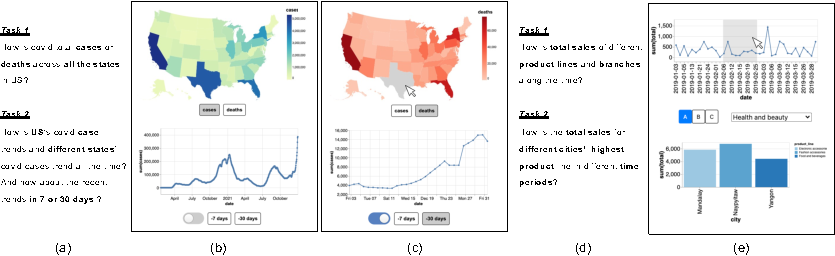
\includegraphics[width=1\textwidth]{figure/fig.pdf}
\vspace*{-2mm}
 \caption{(a) shows two natural language tasks for COVID-19 dataset. (b) is the interface generated for the tasks listed in (a). (c) shows that users can interact with interface to study the deaths distribution by clicking the ``deaths" on the middle buttons and the Texas recent 30 days' trend by clicking the state ``Texas'' on the Map visuallization and clicking the button ``-30 days'' at the bottom.  (d) shows two natural language tasks for a supermarket sales dataset. (e) is the interactive interface generated for tasks in (d).  The top visualization shows the total sales of task 1 where the branch is specified by the button widget and the product line is specified by the dropdown widget. The bottom visualization shows each city's highest product line's sale and the time period is specified by the brushing over the first visualization.  } 
 \label{example}

}

%% Abstract section.
\abstract{
  We propose \sys, the first system to automatically generate interactive multi-visualization interface from natural language tasks.
} % end of abstract

%% ACM Computing Classification System (CCS). 
%% See <http://www.acm.org/about/class> for details.
%% We recommend the 2012 system <http://www.acm.org/about/class/class/2012>
%% For the 2012 system use the ``\CCScatTwelve'' which command takes four arguments.
%% The 1998 system <http://www.acm.org/about/class/class/2012> is still possible
%% For the 1998 system use the ``\CCScat'' which command takes four arguments.
%% In both cases the last two arguments (1998) or last three (2012) can be empty.

%\CCScatlist{
  %\CCScat{H.5.2}{User Interfaces}{User Interfaces}{Graphical user interfaces (GUI)}{};
  %\CCScat{H.5.m}{Information Interfaces and Presentation}{Miscellaneous}{}{}
%}

%% Copyright space is enabled by default as required by guidelines.
%% It is disabled by the 'review' option or via the following command:
% \nocopyrightspace

%%%%%%%%%%%%%%%%%%%%%%%%%%%%%%%%%%%%%%%%%%%%%%%%%%%%%%%%%%%%%%%%
%%%%%%%%%%%%%%%%%%%%%% START OF THE PAPER %%%%%%%%%%%%%%%%%%%%%%
%%%%%%%%%%%%%%%%%%%%%%%%%%%%%%%%%%%%%%%%%%%%%%%%%%%%%%%%%%%%%%%%%

\begin{document}

\maketitle

%% The ``\maketitle'' command must be the first command after the
%% ``\begin{document}'' command. It prepares and prints the title block.

%% the only exception to this rule is the \firstsection command
\section{Introduction}


Interactive visualization interfaces (or simply {\it interfaces}) play a critical role in nearly every stage of data management---including data cleaning~\cite{wu2013scorpion}, wrangling~\cite{Kandel2011WranglerIV}, modeling~\cite{facets}, exploration~\cite{Murray2013TableauYD, Chen2021TSExplainSE}, and communication~\cite{icheck,fivethirtyeight}. 

Such interfaces require considerable expertise and trial-and-error to design and implement because the charts, interactions, and layout should be chosen to support the underlying analysis task~\cite{munzner2014visualization}.
Our recent work \sysold~\cite{chen2022pi2,pi2demo} uses SQL as proxy for analysis task, and is the first system to automatically generate  a fully interactive multi-visualization interface from SQL analysis. Under the hood, \sysold proposes \difftrees as a compact representation of an anlysis task, models interface generation as a schema mapping problem, and search for an optimal interface mapping given a cost model. \sysold helps designer automatically and effectively translate analysis, i.e. SQL queries into interfaces so that user can focus on the analysis without worrying about complicated interface design and implementation. 

Although SQL is ubiquitous in data analysis, it is still hard for normal people, especially non-programmers to write.
Specifying the analysis task in natural language would be a much more accessible and promising way for everyone. Recently, advancements in translation based NLP technologies~\cite{scholak2021picard, https://doi.org/10.48550/arxiv.2109.05153} have vastly improved accuracy of producing schema-aware SQL queries from natural language question. And large task-agnostic language models such as GPT-3\cite{brown2020language} and Codex\cite{chen2021evaluating} can perform well on custom tasks with few-shot examples provided as context. Combined with \sysold, we propose \textbf{ \sys, the first system to automatically generate interactive multi-visualization interface from natural language tasks.} \sys provides Codex with few-shot examples to output \difftree representation from input natural language task and use \sys to generate interactive interface for the input analysis. \yiru{doubel check NLP model description}

Below are two end-to-end examples: 
\begin{example}[Covid Analysis]
Given the COVID-19 dataset, a user is interested in two tasks - ``How is covid total cases or deaths across all the states in US?", and ``How is US‘s covid case trends and different states’ covid cases trend all the time?  And how about the recent trends in 7 or 30 days ? " as shown in \Cref{example}(a). \sys will generate an interactive visualization interface in \Cref{example}(b). The map visualization corresonding to the first task. Users can interact with the middle button widget to choose to show the death distribution in \Cref{example}(c). The line chart in \Cref{example}(b) shows the US overall trend. Users can toggle on to specify the date range e.g. recent 30 days and click on the map visualization to filter specific state, e.g. ``Texas''. After these interactions, \Cref{example}(c)'s bottom line chart shows the Texas' recent 30 days covid cases trend. 
        
\end{example}

\begin{example}[Sales Analysis]
For the supermarket sales dataset~\cite{kagglesales}, in \Cref{example}(d), a user writes two analysis tasks - ``How is total sales of different product lines and branches along the time?'', and ``How is the total sales for different cities‘  highest product line in different time periods?'' \Cref{example}(e) shows the interface where the above visualization shows the total sales of task 1 and the bottom visualization shows each city's highest product line's sale. Notice that the task 2' analysis is a complilcated query analysis which has to first find each city's highest product line in different period and then calculte the total sales. This results in complicated subqueris rather simple SPJA queries. For the interface, users can interact the button widget and the dropdown widget to specify the branch and product line. Brushing over the first visualizaiton will specify the time period for the second analysis task. 
 With such an interactive interface, users can easily explore different branches, product lines and periods. 
        
\end{example}

As we can see,  with \sys, users can purely focus on write analysis task in natural language, and \sys will automatically return a fully interactive multi-visualization interfaces that can perform the data analysis task. 

There is also a line of work which answer natural language task or dialogue  with visualization 

they focus on visualization specification around one certain question, 

\sys is beyond this in that it takes consideration of multi view, it considers interface characteristic 

yet, \sys clearly differ them they mainly focus on single visualization specify /  what's more, since \sys use sql \difftree as intermediate representation, it can express complicated query where these work can not. 



Above all, this paper contribute \sys 

which is able to  
we organize paper in the following 
related work 
system overview 





\section{Related Work}

\subsection{NL to vis }




\subsection{NLP model to SQL}

NLP model to predict sql 

\section{PI2-NL System Design}
\subsection{Design Overview}

\sys defines a concrete set of \difftree syntax as an intermediate representation between natural language tasks and data visualizations. The advantage of \difftree representations over SQL queries is that natural language utterances often contain ambiguities that are hard to be encoded into a single SQL query, and a \difftree is more capable of capturing these ambiguities and is better aligned with \sysold 's visualization interfaces.

For instance, a natural language task "How badly has covid impacted the Seattle area?" could be translated into the following \difftree : select time, ANY(covid\_cases, covid\_deaths) from covid where city = ANY('Seattle', 'Bellevue', 'Tukwila', 'Redmond', 'Tacoma', 'Bothell'); and the two ANY choice nodes could later be mapped to dropdown widgets in the visualization interface. The complete set of \difftree syntax will be discussed in the following section.

\sys leverages the few-shot performance of Codex to produce \difftrees with only a few examples provided in the prompt. We used 50 examples with 5 different database schemata to teach Codex NL-to-\difftree translation. Then, we prompt Codex with a natural language task and the task's database schema to generate a \difftree representation, which would then be used as an input for \sysold to produce interactive data visualizations.

\begin{figure*}
    \centering
    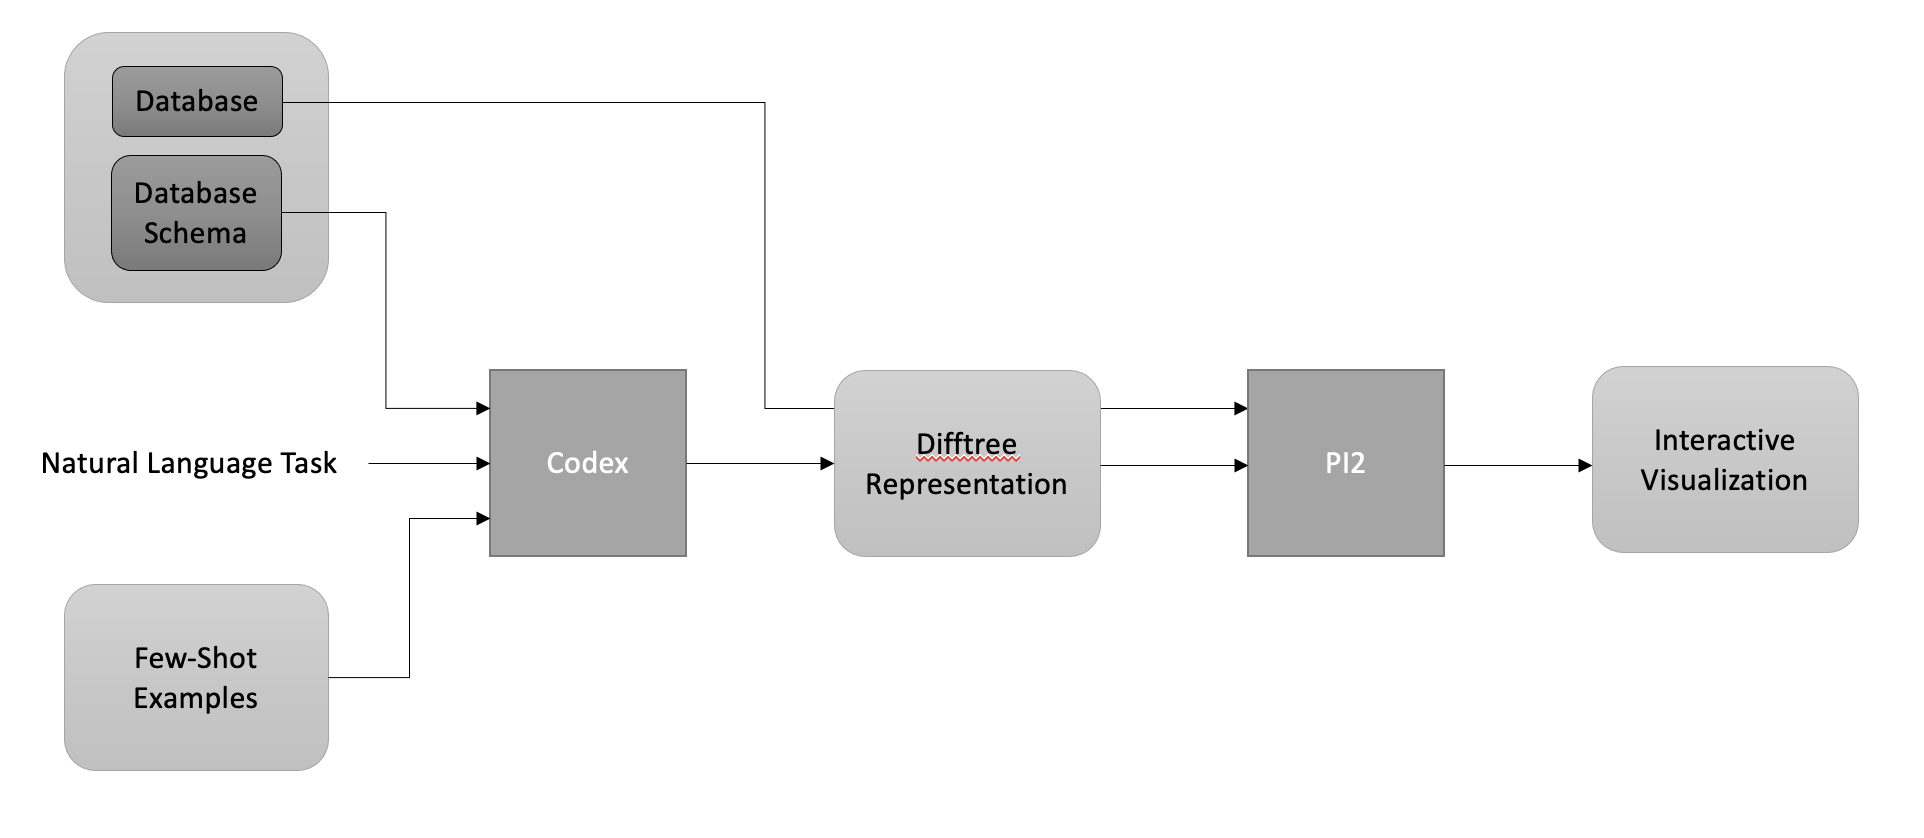
\includegraphics[width=0.8\textwidth]{nlviz-workshop/figure/pipline.png}
    \caption{The complete pipeline for generating interactive interfaces from a natural language task}
    \label{fig:pipline}
\end{figure*}


\subsection{\difftree Representation}

\difftrees were first introduced by PI2\cite{chen2022pi2} to encode the semantic variations among multiple SQL queries. However, there wasn't a well-defined textual representation of \difftree that could be used to transmit among multiple systems. Our paper proposes a formal set of syntax to write a \difftree as text or parse a \difftree from textual input.

\difftree input strings are a strict superset of the traditional SQL language. In addition to the standard SQL syntax, \difftree introduces choice nodes to provide the freedom and capacity to encode more information than a single SQL query. These choice nodes are:

\begin{enumerate}
\item $\mathbf{ANY(c1, ..., ck) \rightarrow c1 \vee ... \vee ck}$. The ANY choice node allows one to select any one of the values enclosed by the parentheses. To specify a range of numeric values, one can instead use $\mathbf{ANY(a - b)}$; e.g., $\mathbf{ANY(3.0 - 5.0)}$ represents any numeric value between 3.o and 5.0. Moreover, it is sometimes beneficial to include a default value in an ANY choice node (e.g., to instruct PI2 setting a default value for a dropdown widget). A default value can be specified by using the 'default' keyword: $\mathbf{ANY(c1, ..., ck, default=ci)}$
\item $\mathbf{SUBSET(c1, ..., ck) \rightarrow c1? \cup ... \cup ck?}$. As the name suggests, the SUBSET choice node specifies a subset of the values listed between the parentheses. For example, the query "select col1, col2 from table1 where $\mathbf{SUBSET(c1, ..., ck)}$" represents all SQL queries that selects col1 and col2 from table1 with any combinations of c1, ..., ck in the where clause.
\item $\mathbf{OPT(t) \rightarrow t \vee NULL}$. The OPT choice node implies that the term in the parentheses is optional in the query. For instance, \difftree query "select col1, col2 from table1 where c1 and $\mathbf{OPT(c2)}$" encodes both SQL query "select col1, col2 from table1 where c1" and "select col1, col2 from table1 where c1 and c2". \difftree query "select col1, OPT(col2) from table1" represents both "select col1 from table1" and "select col1, col2 from table1".
\end{enumerate}

We note that since \difftrees are a strict superset of SQL queries, regular SQL queries are also considered to be valid inputs for the \difftree parser.
\section{Discussion}

Attribute ambiguity
\section{Conclusion}

%\bibliographystyle{abbrv}
\bibliographystyle{abbrv-doi}
%\bibliographystyle{abbrv-doi-narrow}
%\bibliographystyle{abbrv-doi-hyperref}
%\bibliographystyle{abbrv-doi-hyperref-narrow}

\bibliography{ref}
\end{document}
